\chapter{State of the Art} \label{ch:state-of-the-art}

Crafting a comprehensive literature review in an engineering thesis is a meticulous process that involves critically analyzing existing research to contextualize your work within the broader scientific landscape. Start by defining the scope and objectives of your literature review, outlining the key research questions or themes you aim to address. Systematically search and identify relevant peer-reviewed articles, conference papers, and reputable sources related to your topic. As you delve into each source, synthesize the information by identifying common trends, conflicts, gaps, and methodologies used in the field. Organize your review thematically, chronologically, or by grouping similar studies, ensuring a coherent flow of ideas. It's essential to critically evaluate the quality and relevance of each source and discuss their contributions to the field. Through your literature review, you not only showcase your understanding of existing knowledge but also lay the foundation for your engineering thesis by identifying opportunities for innovation and delineating the path forward for your research. \medskip

If these become of significant complexity, overview figures can be applied with great benefit, such as the one shown in~\figref{fig:sota-example}

\begin{figure}[h]
	\begin{small}
		\begin{center}
			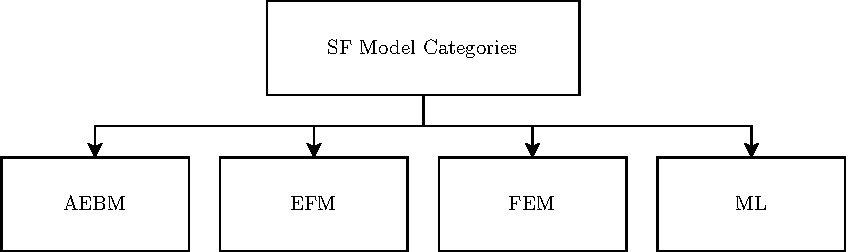
\includegraphics[width=0.8\textwidth]{img/sf-categories.pdf}
		\end{center}
		\caption{Example of sub-category tree.}
		\label{fig:sota-example}
	\end{small}
\end{figure}

This is how to reference the bibliography~\cite{3d-object-pose-estimation-using-stereo-vision-for-object-manipulation-system}. \medskip

This is how to use abbreviations~\gls{anova} or abbreviations with explanations~\gls{cv}.

\section{Problem 1 - Name of Problem 1}\label{sec:lit-rev-problem-1}
literature review of problem 1.

\section{Problem 2 - Name of Problem 2}\label{sec:lit-rev-problem-2}
literature review of problem 2.

\section{Problem 3 - Name of Problem 3}\label{sec:lit-rev-problem-3}
literature review of problem 3.
